\documentclass[11pt]{article}
\usepackage{listings}
\usepackage{graphicx}
\usepackage{color}
\usepackage{amsmath}
\usepackage{amsfonts}

\DeclareMathOperator*{\argmin}{argmin}

\definecolor{codegreen}{rgb}{0,0.6,0}
\definecolor{codegray}{rgb}{0.5,0.5,0.5}
\definecolor{codepurple}{rgb}{0.58,0,0.82}
\definecolor{backcolour}{rgb}{0.95,0.95,0.92}
 
\lstdefinestyle{mystyle}{
    backgroundcolor=\color{backcolour},   
    commentstyle=\color{codegreen},
    keywordstyle=\color{blue},
    numberstyle=\tiny\color{codegray},
    stringstyle=\color{codepurple},
    basicstyle=\footnotesize,
    breakatwhitespace=false,         
    breaklines=true,                 
    captionpos=b,                    
    keepspaces=true,                 
    numbers=left,                    
    numbersep=5pt,                  
    showspaces=false,                
    showstringspaces=false,
    showtabs=false,                  
    tabsize=2
}
 
\lstset{style=mystyle}

\begin{document}
\lstset{language=Matlab}

\title{COMPM012 - Coursework 3}
\author{Esben A. S\o rig}

\maketitle

\section{Practical}

\subsection{k-means implementation}
    \begin{lstlisting}
function [clusterings, centers] = mykmeans(X, k)
    % Randomly initialize centers of clusters
    c = datasample(X, k, 'Replace', false);
    r = repmat(0, size(X, 1), k);
    oldr = 1; % something that is not equal to r initially
    
    dist = @(x, y) norm(x-y);
    
    % Loop as long as the clustering is changing
    while ~isequal(r, oldr)
        oldr = r;
        
        % Assign points to clusters
        for i = 1:size(X,1)
            cluster = 1;
            for j = 1:k
                if dist(X(i, :), c(j, :)) <  dist(X(i, :), c(cluster, :))
                    cluster = j;
                end
            end

            r(i, :) = [repmat(0, 1, cluster-1) 1 repmat(0, 1, k-cluster)];
        end

        % Update center positions
        for i = 1:k
            npoints = 0;
            c(i, :) = 0;
            for j = 1:size(r, 1)
                c(i, :) = c(i, :) + r(j, i)*X(j, :);
                npoints = npoints + r(j, i);
            end
            c(i, :) = c(i, :)/npoints;
        end
    end
    
    centers = c;
    % Output formatting (vector with cluster index for each row in X)
    clustering = repmat(0, size(X,1), 1);
    for i = 1:size(X,1)
       for j = 1:k
           if r(i, j) == 1
                clustering(i) = j;
                break;
           end
       end
    end
   
    clusterings = clustering;
end\end{lstlisting}

\subsection{k-means test on data generated from three gaussians} Firstly, we generate the data and run the k-means algorithm on it.
    \begin{lstlisting}
% Generate data
data = genData2;

% Put data for each cluster in a seperate list
cluster1 = [];
cluster2 = [];
cluster3 = [];
[clusterings, centers] = mykmeans(data, 3);

for i = 1:size(data, 1)
    if clusterings(i) == 1
        cluster1 = [cluster1; data(i, :)];
    end
    if clusterings(i) == 2
        cluster2 = [cluster2; data(i, :)];
    end
    if clusterings(i) == 3
        cluster3 = [cluster3; data(i, :)];
    end
end\end{lstlisting}
    
    We can now plot the clusters the algorithm has found
    \begin{lstlisting}
figure
hold on

scatter(centers(:, 1), centers(:, 2), 200, 'xblack');
scatter(cluster1(:, 1), cluster1(:, 2));
scatter(cluster2(:, 1), cluster2(:, 2));
scatter(cluster3(:, 1), cluster3(:, 2));
legend('Centers', 'Cluster1', 'Cluster2', 'Cluster3');
hold off\end{lstlisting}
    
    \begin{center}
    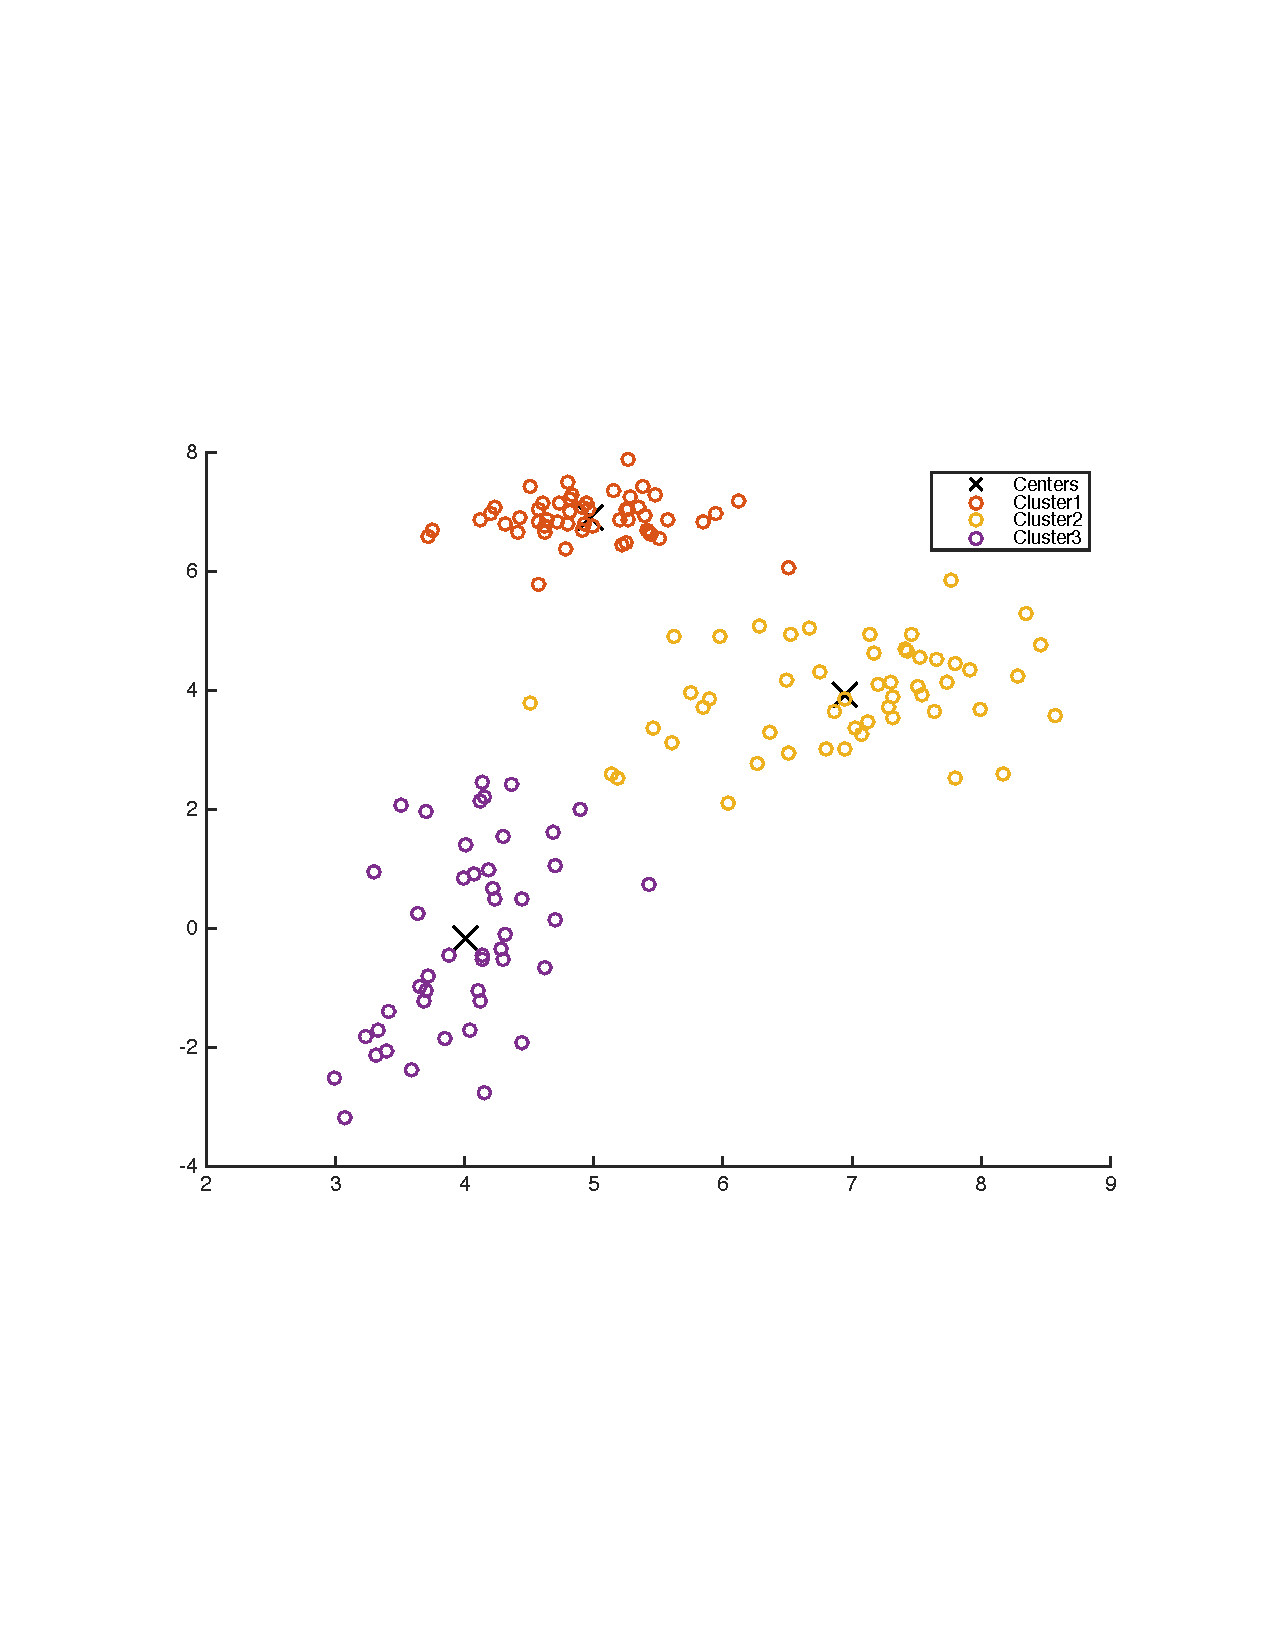
\includegraphics[width=\linewidth]{2-1}
    \end{center}

    
    Comparing this to the true classifications
    \begin{lstlisting}
figure
hold on
scatter(data(1:50, 1), data(1:50, 2));
scatter(data(51:100, 1), data(51:100, 2));
scatter(data(101:150, 1), data(101:150, 2));
legend('True Cluster1', 'True Cluster2', 'True Cluster3');
hold off\end{lstlisting}
    
    \begin{center}
    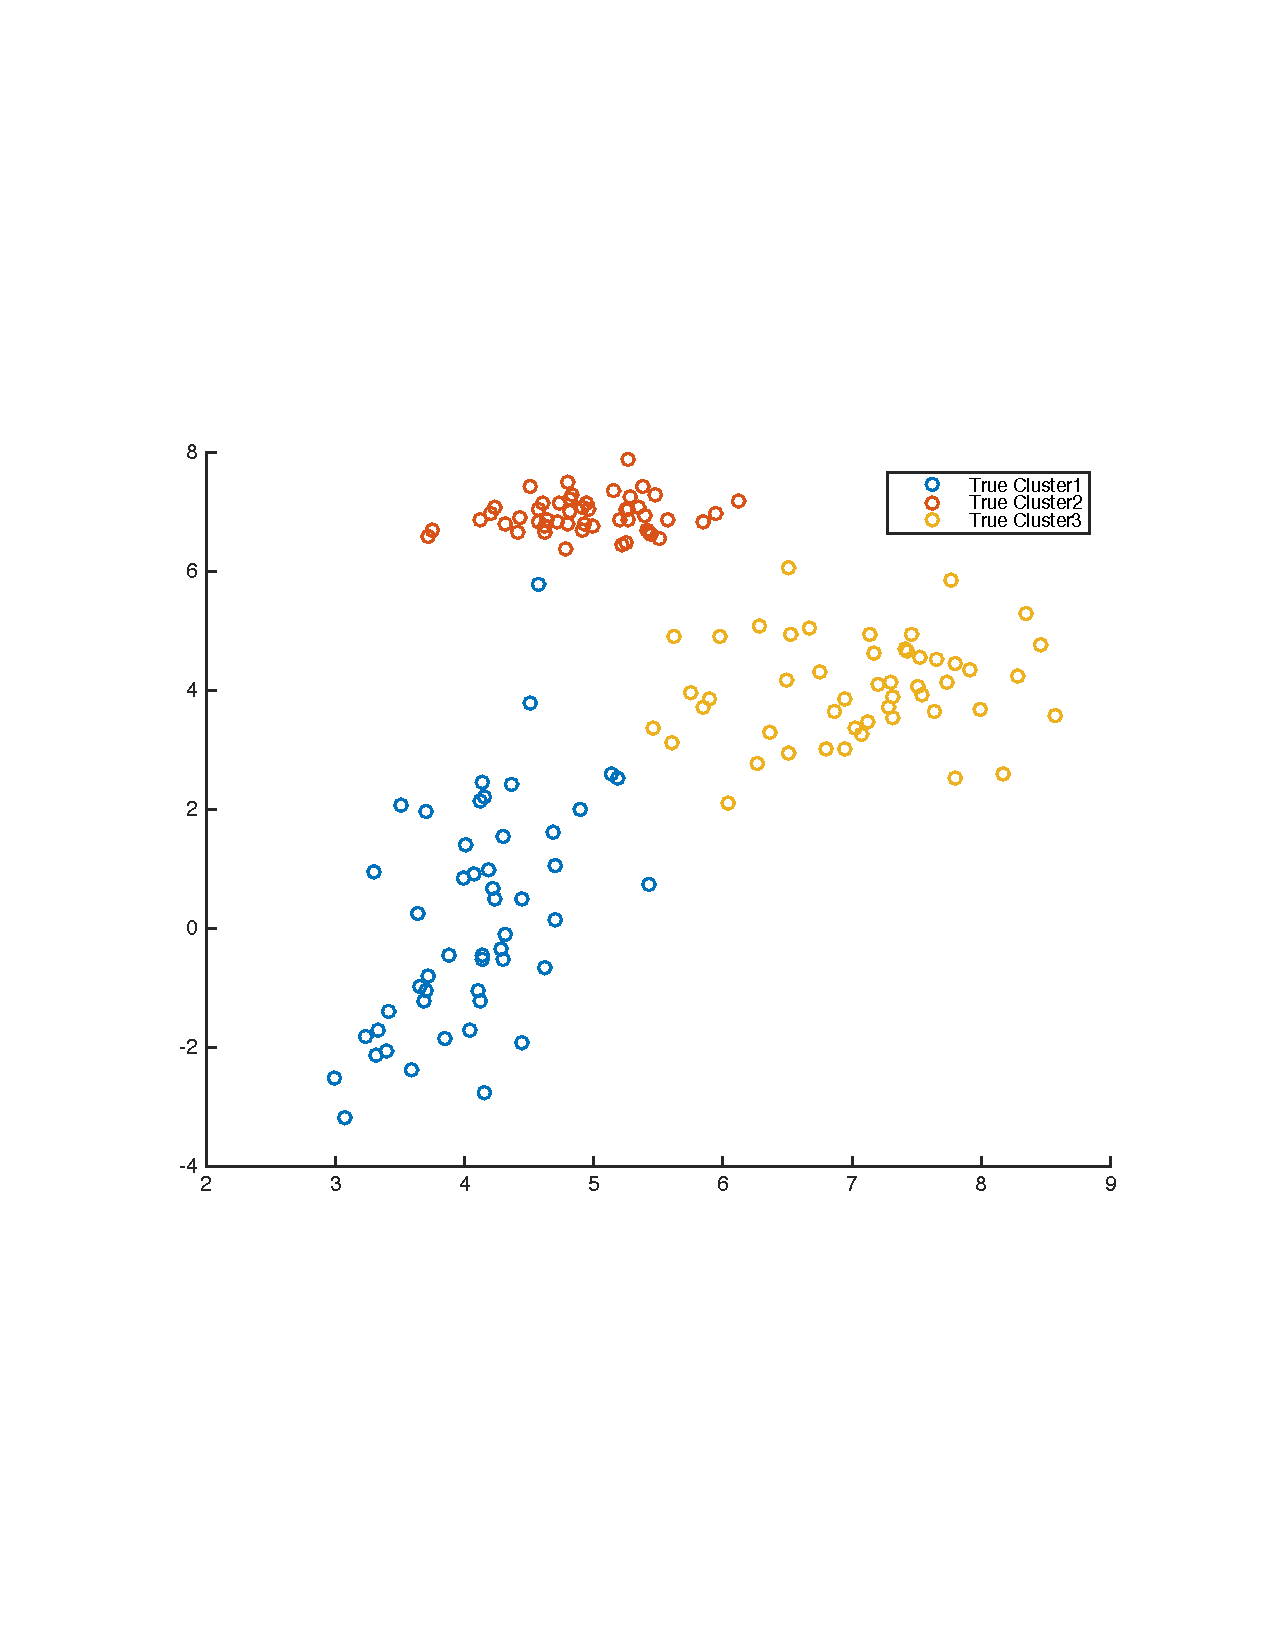
\includegraphics[width=\linewidth]{2-2}
    \end{center}
    
    We clearly get an intuition of how the k-means algorithm is performing on the data. Please see appendix \ref{appendix:movie} for the code that creates the animation of the convergence to a solution for this dataset.
    \par We measure the mean error and standard deviation of the error of the clustering over a 100 runs of the algorithm.
    \begin{lstlisting}
%% Error measurements
errors = [];
for j = 1:100
    [clusterings, centers] = mykmeans(data, 3);
    
    % keep track of the classifications of each true cluster
    firstcluster = [0,0,0];
    secondcluster = [0,0,0];
    thirdcluster = [0,0,0];
    for i = 1:50
        firstcluster(clusterings(i)) = 1 + firstcluster(clusterings(i));
    end
    for i = 51:100
        secondcluster(clusterings(i)) = 1 + secondcluster(clusterings(i));
    end
    for i = 101:150
        thirdcluster(clusterings(i)) = 1 + thirdcluster(clusterings(i));
    end
    % We assume that the mode of the classifications of a true cluster is the class of the true cluster. Therefore, the error of a cluster is the frequency of other classifications appearing for that cluster.
    firstcluster = sort(firstcluster);
    secondcluster = sort(secondcluster);
    thirdcluster = sort(thirdcluster);
    misclassifications = firstcluster(1) + firstcluster(2) + secondcluster(1) + secondcluster(2) + thirdcluster(1) + thirdcluster(2);
    errors = [errors misclassifications/150];
end

meanerror = mean(errors)
stddeviationerror = std(errors)\end{lstlisting}
    
    Which returns:
    \begin{lstlisting}
meanerror =
    0.0333
stddeviationerror =
   2.0922e-17\end{lstlisting}
   
   \subsection{Iris data}
   
   Performing a similar experiment and error measure on the iris dataset is done in a similar way
   
   \begin{lstlisting}
iris = readtable('iris.dat');
params = table2array(iris(:, 1:4));
classifications = table2array(iris(:, 5));
classes = unique(classifications);
class1 = find(strcmp(classifications, classes(1)));
class2 = find(strcmp(classifications, classes(2)));
class3 = find(strcmp(classifications, classes(3)));

errors = [];
for n = 1:100
    clusters = kmeans(params, 3);
    clusters1 = clusters(class1);
    clusters2 = clusters(class2);
    clusters3 = clusters(class3);

    label1 = mode(clusters1);
    label2 = mode(clusters2);
    label3 = mode(clusters3);

    errcount = 0;
    for i = 1:50
        if clusters1(i) ~= label1
            errcount = errcount + 1;
        end
        if clusters2(i) ~= label2
            errcount = errcount + 1;
        end
        if clusters3(i) ~= label3
            errcount = errcount + 1;
        end
    end

    e = errcount/size(params, 1);
    errors = [errors e];
end

mean = mean(errors)
stddeviation = std(errors)\end{lstlisting}

    Which returns
    
    \begin{lstlisting}
mean =
    0.1096
stddeviation =
    0.0117\end{lstlisting}



\section{Questions}
\subsection{Dataset with local minima} We can easily construct a dataset on which our k-means algorithm has local minima. An example of such a dataset is the set $\{ (0,0), (2,0), (-1, 4), (3, 4) \}$. This is clear if we plot the data.
    \begin{lstlisting}
X = [0, 0; 2,0; -1 4; 3 4];

hold on
axis([-2 5 -1 5]);
scatter(X(:, 1), X(:, 2));\end{lstlisting}
    Which gives the plot:
    \begin{center}
    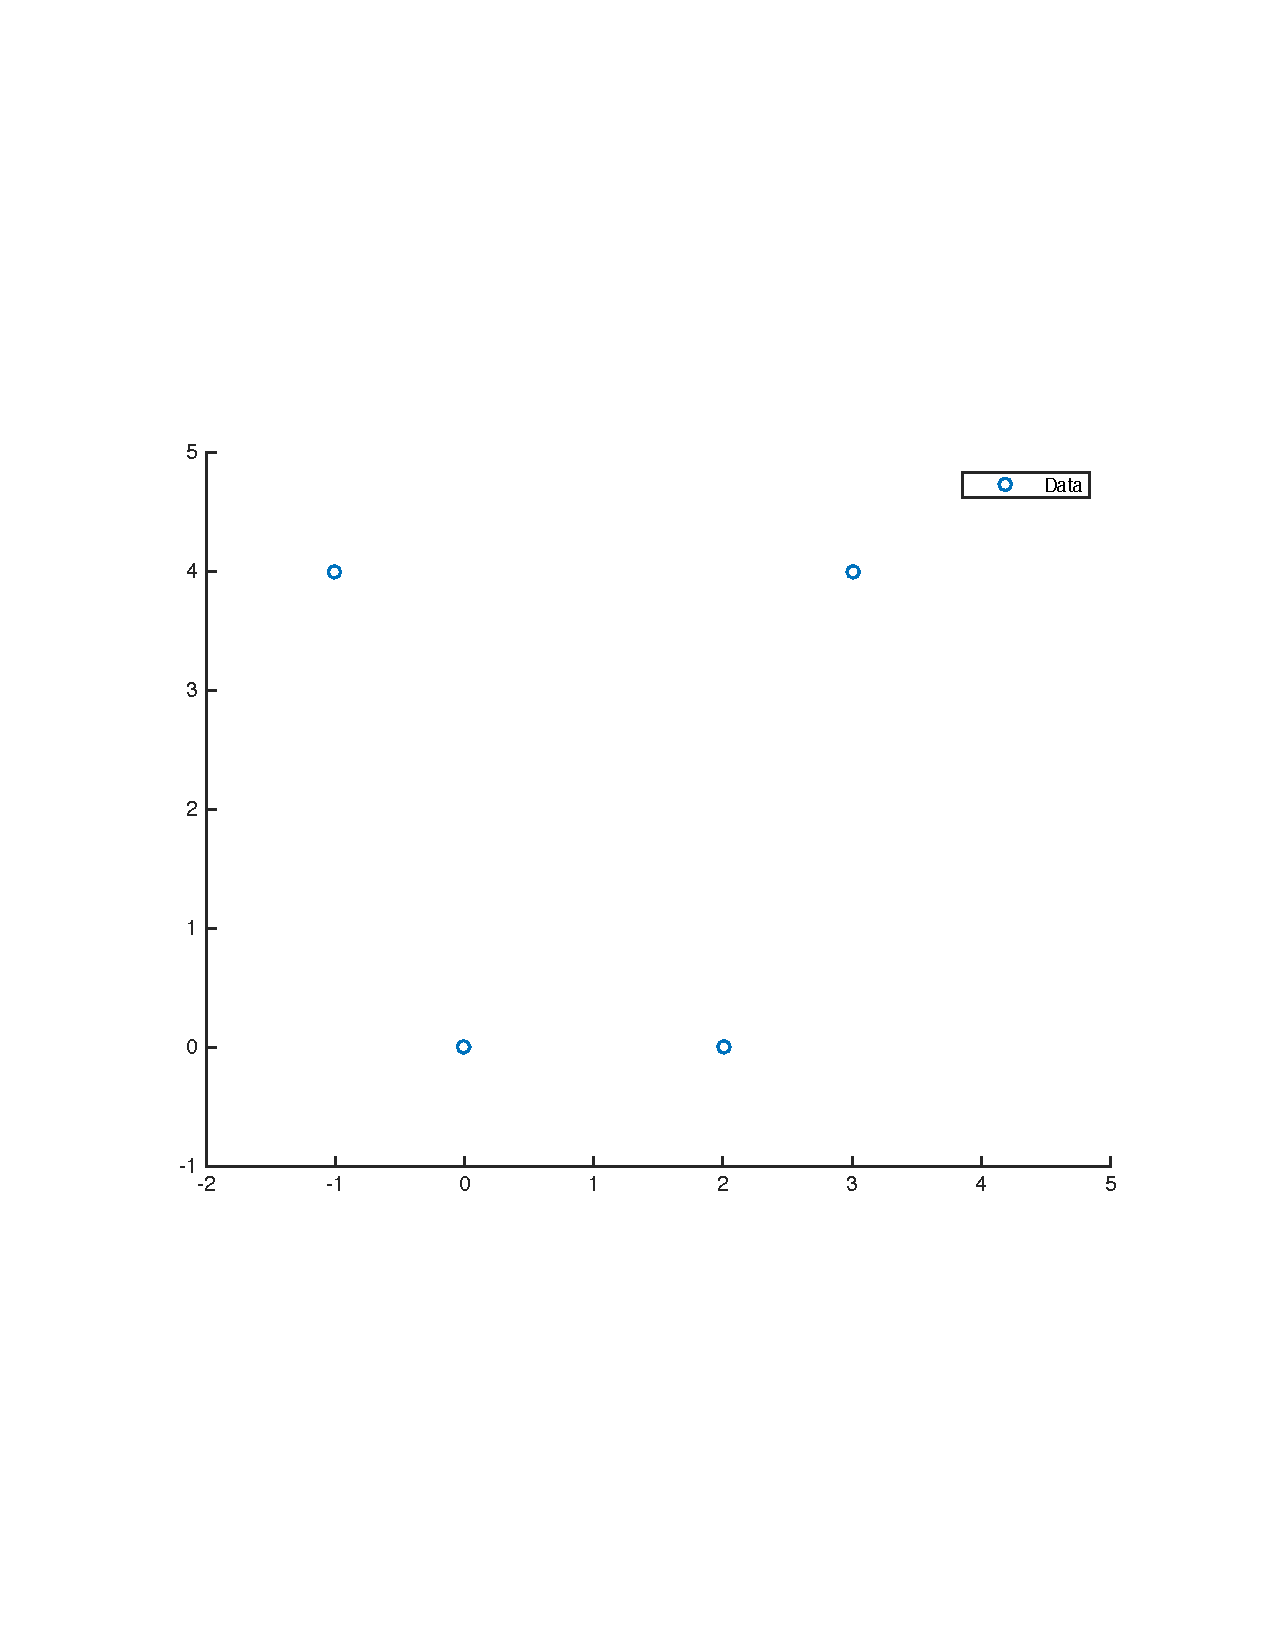
\includegraphics[width=\linewidth]{localminimapoints}
    \end{center}
    
    Running k-means on this dataset will converge in one of two local minima. We run the algorithm twice and plot the centers of the clusters: (in order to get two different results, this code may have to be run several times)
    
    \begin{lstlisting}
[clustering1, centers1] = mykmeans(X, 2);
[clustering2, centers2] = mykmeans(X, 2);
legend('Data');

scatter(centers1(:, 1), centers1(:, 2));
scatter(centers2(:, 1), centers2(:, 2));

legend('Data', 'Minimum 1 centers', 'Miinimum 2 centers');
hold off\end{lstlisting}

    Which produces:
    
    \begin{center}
    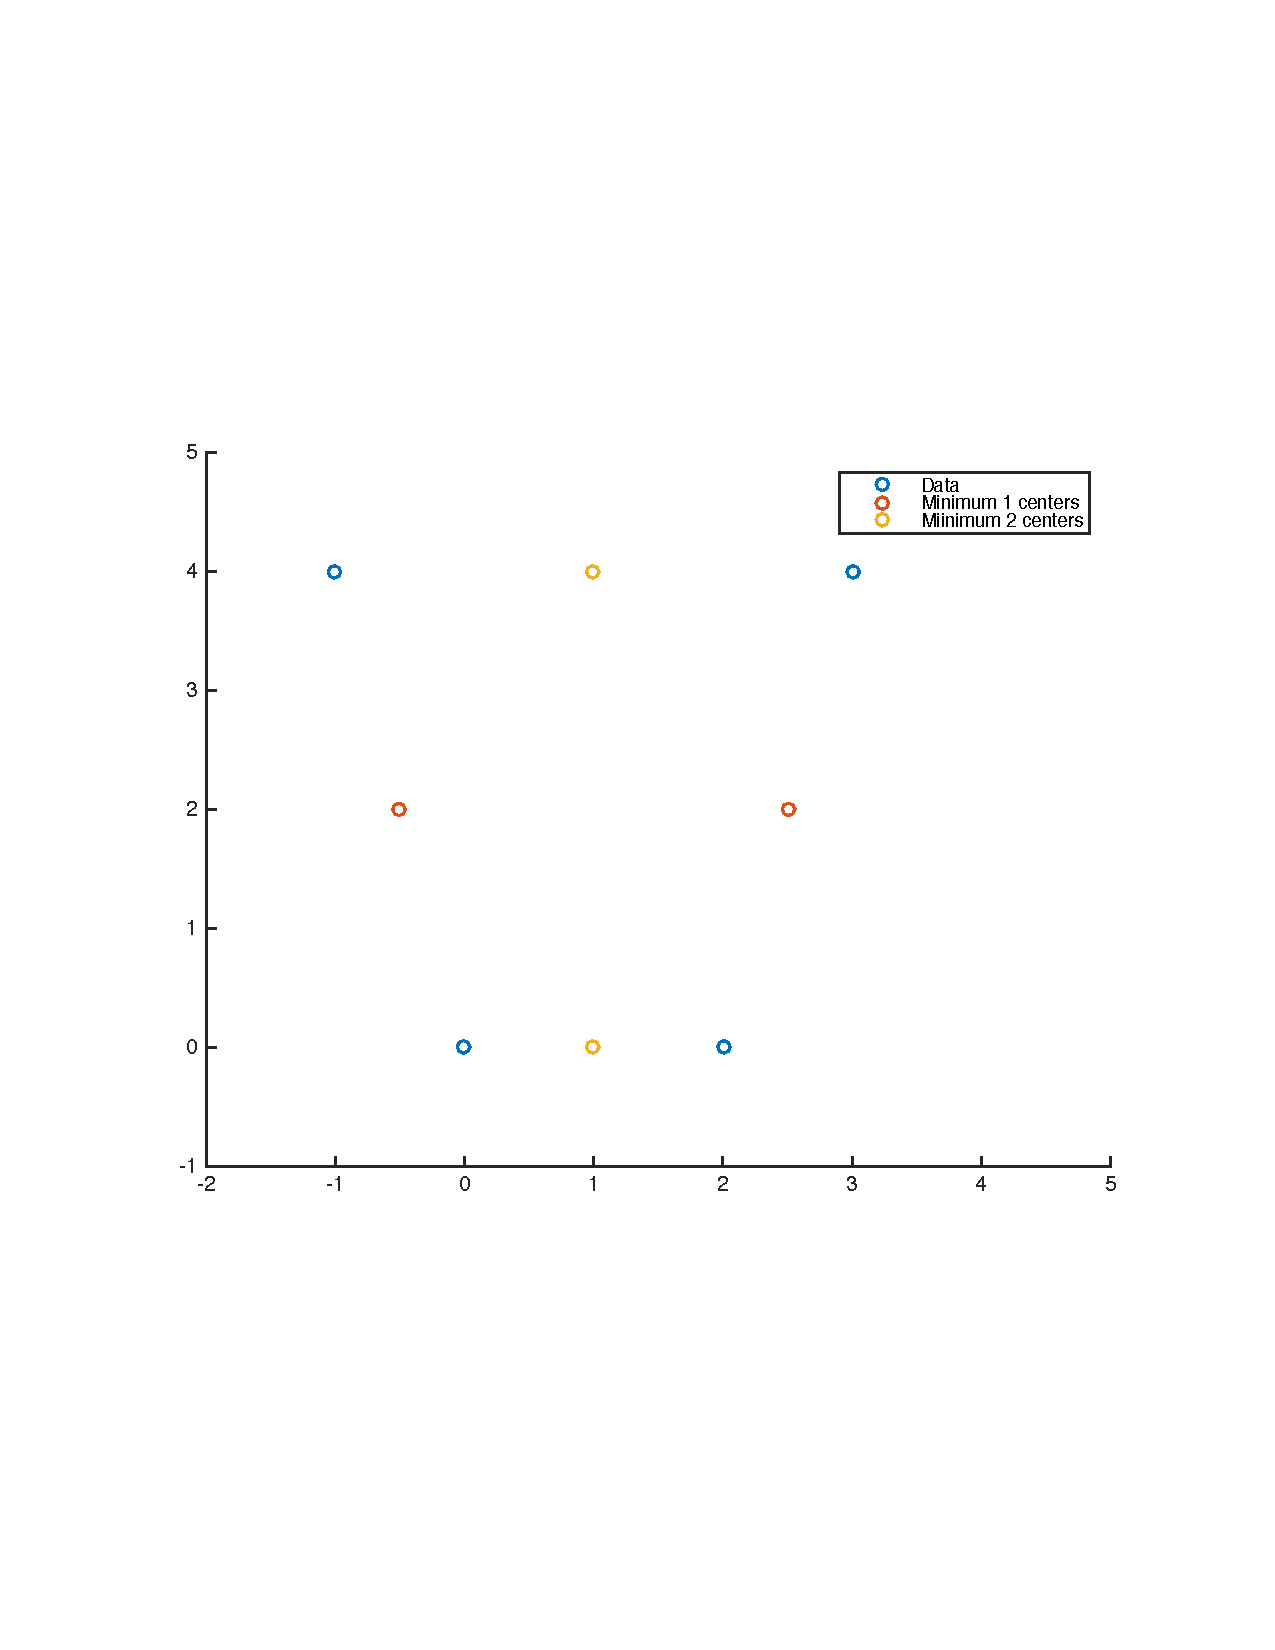
\includegraphics[width=\linewidth]{localminima}
    \end{center}
    
    Here we clearly see the two local minima of the convergence on the four data points.

\subsection{Argument that the centroid is the minimizer of the sum of squared distances}
    We can minimize the summed squared error
    
    \begin{equation}
        SSE = \sum_{i=1}^k \sum_{\mathbf{x} \in C_i} ||\mathbf{x} - \mathbf{c}_i||^2 
        = \sum_{i=1}^k \sum_{\mathbf{x} \in C_i} (\mathbf{x} - \mathbf{c}_i)^2
    \end{equation}
    
    for the $k^{th}$ centroid by setting the derivative with respect to the $k^{th}$ centroid equal to zero.
    
    \begin{equation}
    \begin{split}
        \frac{\delta}{\delta \mathbf{c}_k} \sum_{i=1}^k \sum_{\mathbf{x} \in C_i} (\mathbf{x} - \mathbf{c}_i)^2
        &= \sum_{i=1}^k \sum_{\mathbf{x} \in C_i}  \frac{\delta}{\delta \mathbf{c}_k} (\mathbf{x} - \mathbf{c}_i)^2\\
        &= \sum_{\mathbf{x} \in C_k} 2(\mathbf{x} - \mathbf{c}_k) = 0\\
        \implies \sum_{\mathbf{x} \in C_k} \mathbf{c}_k &= \sum_{\mathbf{x} \in C_k} \mathbf{x}\\
        \implies \mathbf{c}_k &= \frac{1}{\sum_{\mathbf{x} \in C_k} 1} \sum_{\mathbf{x} \in C_k} \mathbf{x}
    \end{split}
    \end{equation}
    
    We see that the minimizer of $\mathbf{c}_k$ is equivalent to the centroid of the cluster.
    
\subsection{Proof of convergence in finite amount of steps}
    We know that the k-means algorithm converges but we do not know if it does so in finitely or infinitely many steps. Here we show that the k-means algorithm does indeed converge in finitely many steps.
    \par \textbf{Proof:} The k-means algorithm stops once there is no longer any improvement in the clustering. It will therefore never reach the same clustering twice. Each possible k-clustering of the input consists of k subsets. The number of subsets of the input is a finite number and the number of k subsets of the input is bounded above by this. Consequently, there is a finite number of possible clusterings. Hence the k-means algorithm will terminate after a finite number of iterations.
\section{Extension}
\subsection{k-means segmentation}

    The objective of the algorithm is to find the segmentation $\{i_1, ..., i_{k-1}\}$ of a sequence of points $\{\mathbf{x}_1, ..., \mathbf{x}_l\} \in \mathbb{R}^n$ that is the global minimum of the following optimisation problem:
    
    \begin{equation}
        \argmin_{i_1, ..., i_{k-1}; \mathbf{c}_1, ..., \mathbf{c}_k} \sum_{j=1}^k \sum_{p=i_{j-1} + 1}^{i_j} ||\mathbf{x}_p - \mathbf{c}_j ||^2
    \end{equation}
    
    The algorithm must run in polynomial time in $l$, $n$, and $k$. We start by defining the error function as it will be useful when searching for minima of in the error.
    
    \begin{lstlisting}
function e = error(delimiters, X)
    e = 0;
    bounddelimiters = [0 delimiters size(X, 1)];
    for j = 2:size(bounddelimiters, 2)
        indeces = (1+bounddelimiters(j-1)):bounddelimiters(j);
        segment = X(indeces, :);
        centroid = sum(segment)/size(segment, 1);
        for k = 1:size(segment, 1)
            e = e + norm(segment(k, :)-centroid)^2;
        end
    end
end\end{lstlisting}
    
    We can now proceed to designing  the segmentation algorithm. 
    Let $\mathbf{i}^*_{n, k}$ be the set of segment delimiters $\{ i^*_1, ..., i^*_{k-1} \}$ that minimises the error of segmenting the points $x_1, ..., x_n$ into $k$ segments. The key observation for construction of a polynomial time algorithm is that $\mathbf{i}^*_{n,k}$ can be described as
    \begin{equation}
    \begin{split}
        \mathbf{i}^*_{n,k} &= \mathbf{i}^*_{j, k-1} \cup \{ j \} \text{ where } \\
        j &= \argmin_{1 \leq j < n} (E(\mathbf{i}^*_{j, k-1} \cup \{ j \} ))
    \end{split}
    \end{equation}
    
    Here $E$ denotes the error function of the segmentation produced a set of delimiters. From this observation we can construct a dynamic programming algorithm that builds a matrix of the optimal segmentations and a matrix of their errors. When the algorithm has reached the optimal segmentation $\mathbf{i}^*_{n,k}$ we have found the solution. The Matlab implementation of the algorithm is listed here:
    
    \begin{lstlisting}
function delimiters = segmentation(X, k)
    % E(i, k) represents the minimum error of segmenting
    % X(1:i, :) into k segments.
    E = [];
    
    % D(i, j) stores the jth delimiter that segments X(1:i, :)  
    % into the optimal j+1 segments.
    D = [];
    
    % We initialise E's first column (error of a single 
    % segment over the points X(1:i, :))
    for i = 1:size(X, 1)
        E(i,1) = error([], X(1:i, :));
    end
    
    % We then proceed to filling out each entry in E until
    % we have reached our objective (the minimum k 
    % segmentation of all points in X).
    for i = 1:size(X, 1)
        for l = 2:min(i, k)
            % Find min error of segmenting x_1, ..., x_i 
            % into l segments
            minerror = Inf;
            for j = 1:(i-1)
                if j >= l
                    e = E(j, l-1) + error([], X((j+1):i, :));
                    if e < minerror
                        minerror = e;
                        D(i, l) = j; % Store delimiter
                    end
                end
            end
            E(i, l) = minerror;
        end
    end
    
    % We retrieve the optimal delimiters from D
    delimiters = [];
    delimiter = size(X, 1);
    for i = k:-1:2
       delimiter = D(delimiter, i);
       delimiters = [delimiters delimiter];
    end
    delimiters = sort(delimiters)
end\end{lstlisting}

    \textbf{Informal argument of time complexity}: The running time is polynomial in $l$, $n$, and $k$ since the algorithm simply consists of nested loops running over $l$ and $k$. In the inner most loop, the error function is called, which is similarly polynomial in complexity in $k$ and $l$ but also $n$ (since we sum over the points). The complexity of the algorithm can therefore be bounded above by a constant multiple of some polynomial in $n$, $l$, and $k$.
    

\subsection{(p, k)-means}
    
    We derive the minimiser of the objective for each $C_i$ in the same way as with the squared distance. We let the derivative with respect to $\mathbf{c}_k$ be equal to zero and solve for $\mathbf{c}_k$. We start by finding the derivative with respect to $\mathbf{c}_k$. 
    
    \begin{equation} \label{eq:5}
        \frac{\delta}{\delta \mathbf{c}_k} \sum_{i=1}^k \sum_{\mathbf{x} \in C_i} d_p (\mathbf{c}_i, \mathbf{x}) = \sum_{\mathbf{x} \in C_k} \frac{\delta}{\delta \mathbf{c}_k} d_p(\mathbf{c}_k, \mathbf{x})
    \end{equation}
    
    We assume that the components of the inputs are nonnegative and obtain
    \begin{equation}
    \begin{split}
        \frac{\delta}{\delta \mathbf{c}_k} d_p(\mathbf{c}_k, \mathbf{x}) &= \frac{\delta}{\delta \mathbf{c}_k} (\sum_{i=1}^n \mathbf{c}_{k,i}^p - \mathbf{x}_i^p - p(\mathbf{c}_{k,i} - \mathbf{x}_i) \mathbf{x}_i^{p-1} )\\
        &= p \mathbf{c}_k^{p-1} - p \mathbf{x}^{p-1}
    \end{split}
    \end{equation}
    
    Where $\mathbf{x}^n$ denotes that each component of $\mathbf{x}$ is raised to the $n$th power. Inserting back in (\ref{eq:5}) and setting this equal to zero, we can now solve for $\mathbf{c}_k$
    
    \begin{equation}
    \begin{split}
        \sum_{\mathbf{x} \in C_k} (p \mathbf{c}_k^{p-1} - p \mathbf{x}^{p-1}) &= 0\\
        \implies \sum_{\mathbf{x} \in C_k} \mathbf{c}_k^{p-1} &= \sum_{\mathbf{x} \in C_k} \mathbf{x}^{p-1}\\
        \implies \mathbf{c}_k &= \sqrt[p-1]{\frac{\sum_{\mathbf{x} \in C_k} \mathbf{x}^{p-1}} {|C_k|}}
    \end{split}
    \end{equation}
    
    Observe that this result is consistent with our result for the euclidean distance. We can now design the $(p, k)$-means algorithm.
    
    \begin{enumerate}
        \item \textbf{for} $i = 1, ..., k$ \textbf{do}
        \begin{equation*}
            C_i = \{ \mathbf{x} \in x \mid i = \argmin_{1 \leq j \leq k} d_p(\mathbf{c}_j, \mathbf{x}) \}
        \end{equation*}
        
        \item \textbf{for} $j = 1, ..., k$ \textbf{do}
        \begin{equation*}
            \mathbf{c}_j = \sqrt[p-1]{\frac{\sum_{i=1}^l r_{ij} \mathbf{x}_i^{p-1}}{\sum_{i=1}^l r_{ij}}}
        \end{equation*}
        
        \item \textbf{While} not converged \textbf{go to} step 1.

    \end{enumerate}

    Again, $\mathbf{x}^n$ denotes that each component of $\mathbf{x}$ is raised to the $n$th power and $\sqrt[n]{\mathbf{x}}$ denotes that we take the $n$th root of each component of x. The argument of convergence for this algorithm is similar to the argument for the standard $k$-means algorithm. That is, the objective decreases in step 1 and 2 and the objective is bounded below. Hence the algorithm converges. 

\section{Appendix}
    \subsection{Movie generation code} \label{appendix:movie}
        \begin{lstlisting}
%% Movie
X = data;
k = 3;
% Randomly initialize centers of clusters
c = datasample(X, k, 'Replace', false);
r = repmat(0, size(X, 1), k);
oldr = 1; % something that is not equal to r initially
movie = [];

dist = @(x, y) norm(x-y);

% Loop as long as the clustering is changing
while ~isequal(r, oldr)
    oldr = r;
    
    % Assign points to clusters
    for i = 1:size(X,1)
        cluster = 1;
        for j = 1:k
            if dist(X(i, :), c(j, :)) <  dist(X(i, :), c(cluster, :))
                cluster = j;
            end
        end

        r(i, :) = [repmat(0, 1, cluster-1) 1 repmat(0, 1, k-cluster)];
    end
    
    %MOVIE GENERATION
    % Split the data into the three clusters
    cluster1 = [];
    cluster2 = [];
    cluster3 = [];

    for i = 1:size(X, 1)
        if r(i,1) == 1
            cluster1 = [cluster1; X(i, :)];
        end
        if r(i,2) == 1
            cluster2 = [cluster2; X(i, :)];
        end
        if r(i,3) == 1
            cluster3 = [cluster3; X(i, :)];
        end
    end
    
    % Plot the centers and the three clusters
    hold on
    scatter(c(:, 1), c(:, 2), 200, 'xblack');
    if size(cluster1, 1) ~= 0
        scatter(cluster1(:, 1), cluster1(:, 2));
    end
    if size(cluster2, 1) ~= 0
        scatter(cluster2(:, 1), cluster2(:, 2));
    end
    if size(cluster3, 1) ~= 0
        scatter(cluster3(:, 1), cluster3(:, 2));
    end
    legend('Centers', 'Cluster1', 'Cluster2', 'Cluster3');
    hold off
    movie = [movie getframe];
    clf;
    % MOVIE GENERATION OVER

    % Update center positions
    for i = 1:k
        npoints = 0;
        c(i, :) = 0;
        for j = 1:size(r, 1)
            c(i, :) = c(i, :) + r(j, i)*X(j, :);
            npoints = npoints + r(j, i);
        end
        c(i, :) = c(i, :)/npoints;
    end
end
movie2avi(movie, 'k-means.avi', 'fps', 1);\end{lstlisting}





\end{document}
